\section{Introduction}
\label{sec:introduction}
% questioning the how

% Rise of DL
In recent years, deep learning models have demonstrated superior performance on a variety of tasks \cite{ruede2020multi, brinker2019deep, nguyen2020super}. While performance is still increasing and more tasks are being handled, their performance comes at the cost of complexity: models often use millions to billions of parameters to achieve universal function approximation.
This complexity means that they remain black boxes that cannot be interpreted even by experts.

% rise of XAI
Such a black box is able to predict well for unseen yet similar data, answering the question of \textit{what} is the most likely label for an input sample. 
However, most models will provide no answer to \textit{why} the model chose this label for the instance and which features of the instance were crucial for making this prediction. 

For instance, withing object recognition one would likely assume that the presence (or absence) of an object in the image causes a model to decide for a specific object category, closely akin to how humans base their decision process. As seen in \autoref{fig:bb}, the presence of the cat in the input image $\mathbf{x}$ should be causing the model to predict the label 'cat'.  

\begin{figure}[t]
    \centering
    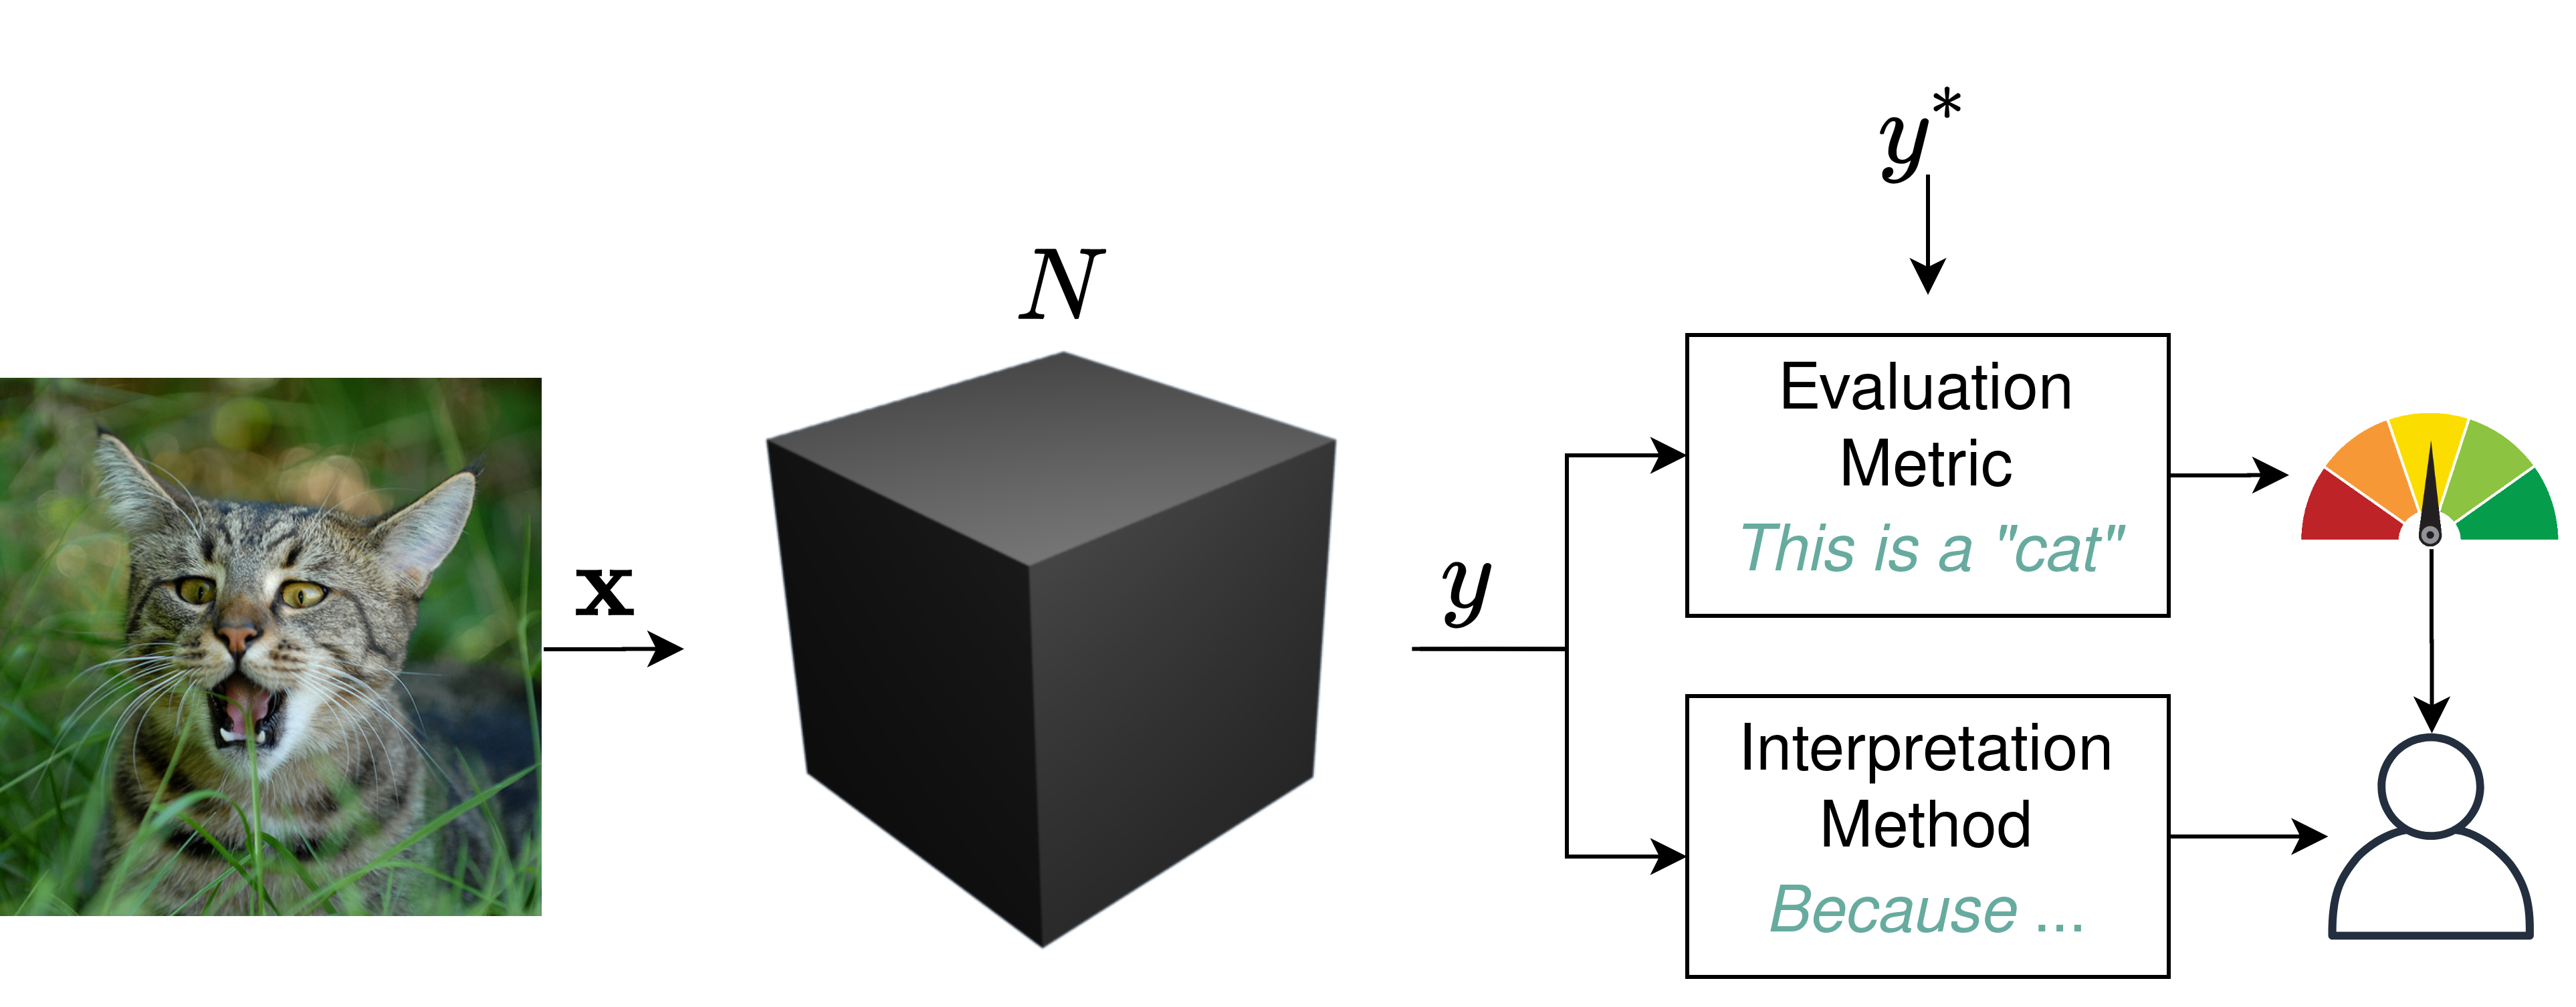
\includegraphics[width=\linewidth]{figures/bb_cat.png}
    \caption{Prediction pipeline using a machine learning model, depicted as blach box. Typically, evaluation metrics require the prediction $y$ and the ground truth label $y^*$ allowing for the assessmant of the model's accuracy. Additionally answering the question \textit{why}, i.e. making the model interpretable for a human, requires additional methods.}
    \label{fig:bb}
    \vspace{-0.3cm}
\end{figure}

Automated algorithms are already in use in critical areas, such as medicine TODOcite, the criminal justice system \cite{chouldechova2017fair} and the financial sector TODOcite or the piloting of self-driving cars.
Thus, as machine learning models are moving out of the lab into the real-world, the inability of humans to understand these models seems even more problematic. 

Thus, automated interpretation methods are required to make sense of the reasoning process and robustness of such deep learning based models and to ensure that a model makes decisions without unfair or hidden biases. 
The research field approaching the explanation or validation of machine learning models is called explainable artificial intelligence (XAI).


%  not knowing why models decide
Not knowing about the biases of a network the vastly advancing technology of machine learning to be used in high-stakes and safety critical applications and prevent real-life deployment of such systems. 
Furthermore, the rise in machine learning model deployments also caused the development of adversarial attacks. These attacks attempt to fool a machine learning model by providing deceptive input. Fooling refers to the resulting malfunction of the model. 
% TODO first example



% security aspect of nns

% Importance of interpretability: hidden biases --> cannot be deployed in real world


% ethical examples: decisions where it is most crucial to have working systems

% Broadness of research field

% Outline of paper

% https://towardsdatascience.com/interpretability-in-machine-learning-70c30694a05f 
% biases in ml models - boils down to data


% For instance, withing object recognition one would like to assume that the presence (or absence) of an object in the image causes a model to decide for a specific object category, closely akin to how humans base their decision process. 





% sort of prove that neural networks make a safe decision without biases

% much broader context to create security and large scale applications 

% https://dl.acm.org/doi/pdf/10.1145/3387514.3405859?casa_token=lCc16GOTZsEAAAAA:gypLNU1o2Wwl3wt_b8stRbb0mgxEomX8PWprPeciNdkhVften3-5E01RM50e0W9NGQaGd4TrLOhA

% explainability can be viewed as an active characteristic of a model, denoting any action orprocedure taken by a model with the intent of clarifying or detailing its internal functions.


In particular, it is unclear how the variety of proposed model interpretation methods are related and what common concepts can be used to evaluate and compare them. 
Many works are dedicated to establish a formal definition of what it means to be interpretable, and how to select, evaluate and compare methods for generating explanations of machine learning models. \cite{murdoch2019definitions, lipton2018mythos}.



Not knowing about attacks and data arranged to exploit specific vulnerabilities has contributed to a relatively new research field of XAI comprising topics of (1) \textit{model explanations}, (2) \textit{adversarial attacks}, or manipulation methods and (3) the field of \textit{adversarial manipulations of model explanations}. All of this is also known by the name of robust machine learning or even explainable artificial intelligence, as all subfields have the common goal to make models more robust and safe for deployment. 
(1) refers to the development of techniques that can be used to understand and explain the decision making process of a machine learning model or even the development of models that are inherently interpretable. (2) is the field of detecting vulnerabilites in models that cause models to be deceived by altered input. 
(3) is the main topic of this paper, i.e. how to fool explanation models in order to detect vulnerabilities and malfunctions in explanation methods. 

Detecting such vulnerabilities in models is most crucial 

Fragility limits how much wecan trust and learn from the interpretations



% While most of the approaches to explainability focus on the application to computer vision tasks, other domains are seldomly chosen. 
Most research on explainability focuses on the application of computer vision tasks. 
% todo cite a lot here
% https://www.bmc.com/blogs/machine-learning-interpretability-vs-explainability/ 7

% Visually appealing methods and easiy visual assessment of results. 
Most works in the field of XAI focus on image classification tasks, mostly because visualizations of a neural networks prediction can be easily verified by a human. The general purpose of image classification is to detect what objects are in an image. If a model works can be checked rather easily (if an image contains a cat, the prediction of a neural network should be cat and not some other object category). However, how it works (\textit{interpretability}), i.e. based on which features in the image the decision is made or which parameters in the model influence the prediction most, is an entirely different matter (\textit{explainability}).  


More importantly, while a big motivation for the development of robust and explainable systems is to overcome biases in models, datasets with direct implication of biases are seldomly used and by far not treated as benchmarking scenarios for explainability analyses.  


% Theoretical background
% why do adv attacks make sense? most models are trained on iid samples and thus not directly applicable to the real world, as the real world violates this statistical assumption. 




% Outline
The overview presented in this article examines the existing literature and contributions in the field of XAI focusing on methods to manipulate explanation methods.  
The critical literature analysis might serve as a motivation and step towards the biggest problems in XAI: How to make sure that interpretations of models are truly valid. 
This paper is structured as follows... 
